\begin{sidewaystable}[]
\centering
\begin{tabular}{|c|c|c|c|c|c|c|}
\hline
\multicolumn{7}{|c|}{Th1} \\
 \hline
        Study & $\alpha$ CD3 & $\alpha$ CD28 & IL-2 & IL-12 & TNF-$\alpha$ & $\alpha$ IL-4\\
        \hline
        Field 2020 \cite{Field2020} & 5 $\mu$g/mL & 0.5 $\mu$g/mL & 100 U/mL & 10 ng/mL & 10 $\mu$g/mL & \textemdash\\
        Bailis 2019 \cite{Bailis2019} & beads & beads & 5 ng/mL & 2 ng/mL & 10 $\mu$g/mL & \textemdash\\
        Sallin 2017 \cite{Sallin2017} & 3 $\mu$g/mL & 1 $\mu$g/mL & 0.12-30 ng/mL & 0.12-30 ng/mL & 10 $\mu$g/mL & \textemdash\\
        Yang 2019 \cite{Yang2019} & 1 $\mu$g/mL & 1 $\mu$g/mL & \textemdash & 10 ng/mL & 5 $\mu$g/mL & 100 ng/mL\\
        Thomas 2012 \cite{Thomas2012} & 1 $\mu$g/mL & 1 $\mu$g/mL & \textemdash & 10 ng/mL & 10 $\mu$g/mL & \textemdash\\
        Jiang 2018 \cite{Jiang2018} & 5 $\mu$g/mL & 5 $\mu$g/mL & \textemdash & 10 ng/mL & 10 $\mu$g/mL & \textemdash\\
        Pham 2014 \cite{Pham2014} & 2 $\mu$g/mL & 0.5 $\mu$g/mL & \textemdash & 5 ng/mL & 10 $\mu$g/mL & \textemdash\\
        Wagner 2021 \cite{Wagner2021} & 1 $\mu$g/mL & 1 $\mu$g/mL & \textemdash & 20 ng/mL & \textemdash & \textemdash\\
        Puleston 2021 \cite{Puleston2021} & 5 $\mu$g/mL & 2 $\mu$g/mL & 100 U/mL & 10 ng/mL & 4 $\mu$g/mL & \textemdash\\
        \hline
        \multicolumn{7}{|c|}{Th2} \\
        \hline
        Study & $\alpha$ CD3 & $\alpha$ CD28 & IL-2 & IL-4 & $\alpha$ IL-12 & $\alpha$ IFN$\gamma$\\
        \hline
        Field 2020 \cite{Field2020} & 5 $\mu$g/mL & 0.5 $\mu$g/mL & 100 U/mL & 10 ng/mL & 10 $\mu$g/mL & 10 $\mu$g/mL\\
        Angela 2016 \cite{Angela2016} & \textemdash & \textemdash & 25 U/mL & 10 U/mL & \textemdash & 1 $\mu$g/mL\\
        Thomas 2012 \cite{Thomas2012} & 1 $\mu$g/mL & 1 $\mu$g/mL & \textemdash & 40 ng/mL & 10 $\mu$g/mL & 10 $\mu$g/mL\\
        Jiang 2018 \cite{Jiang2018} & 5 $\mu$g/mL & 5 $\mu$g/mL & \textemdash & 10 ng/mL & \textemdash & 10 $\mu$g/mL\\
        Pham 2014 \cite{Pham2014} & 2 $\mu$g/mL & 0.5 $\mu$g/mL & \textemdash & 10 ng/mL & \textemdash & 10 $\mu$g/mL\\
        Wagner 2021 \cite{Wagner2021} & 1 $\mu$g/mL & 1 $\mu$g/mL & \textemdash & 20 ng/mL & \textemdash & \textemdash\\
        Puleston 2021 \cite{Puleston2021} & 5 $\mu$g/mL & 2 $\mu$g/mL & 100 U/mL & 10 ng/mL & \textemdash & 4 $\mu$g/mL\\
        \hline
\end{tabular}
\caption{\textbf{Table summary of CD4+ polarization conditions} A meta-analysis of various studies with \textit{in vitro} CD4+ subset polarization condition protocols. Included are the polarization conditions for Th1s and Th2s across 10 studies. Units are presented as described in the original studies.}
\label{tab:CD4polarizationSupp}
\end{sidewaystable}

\begin{figure}
    \centering
    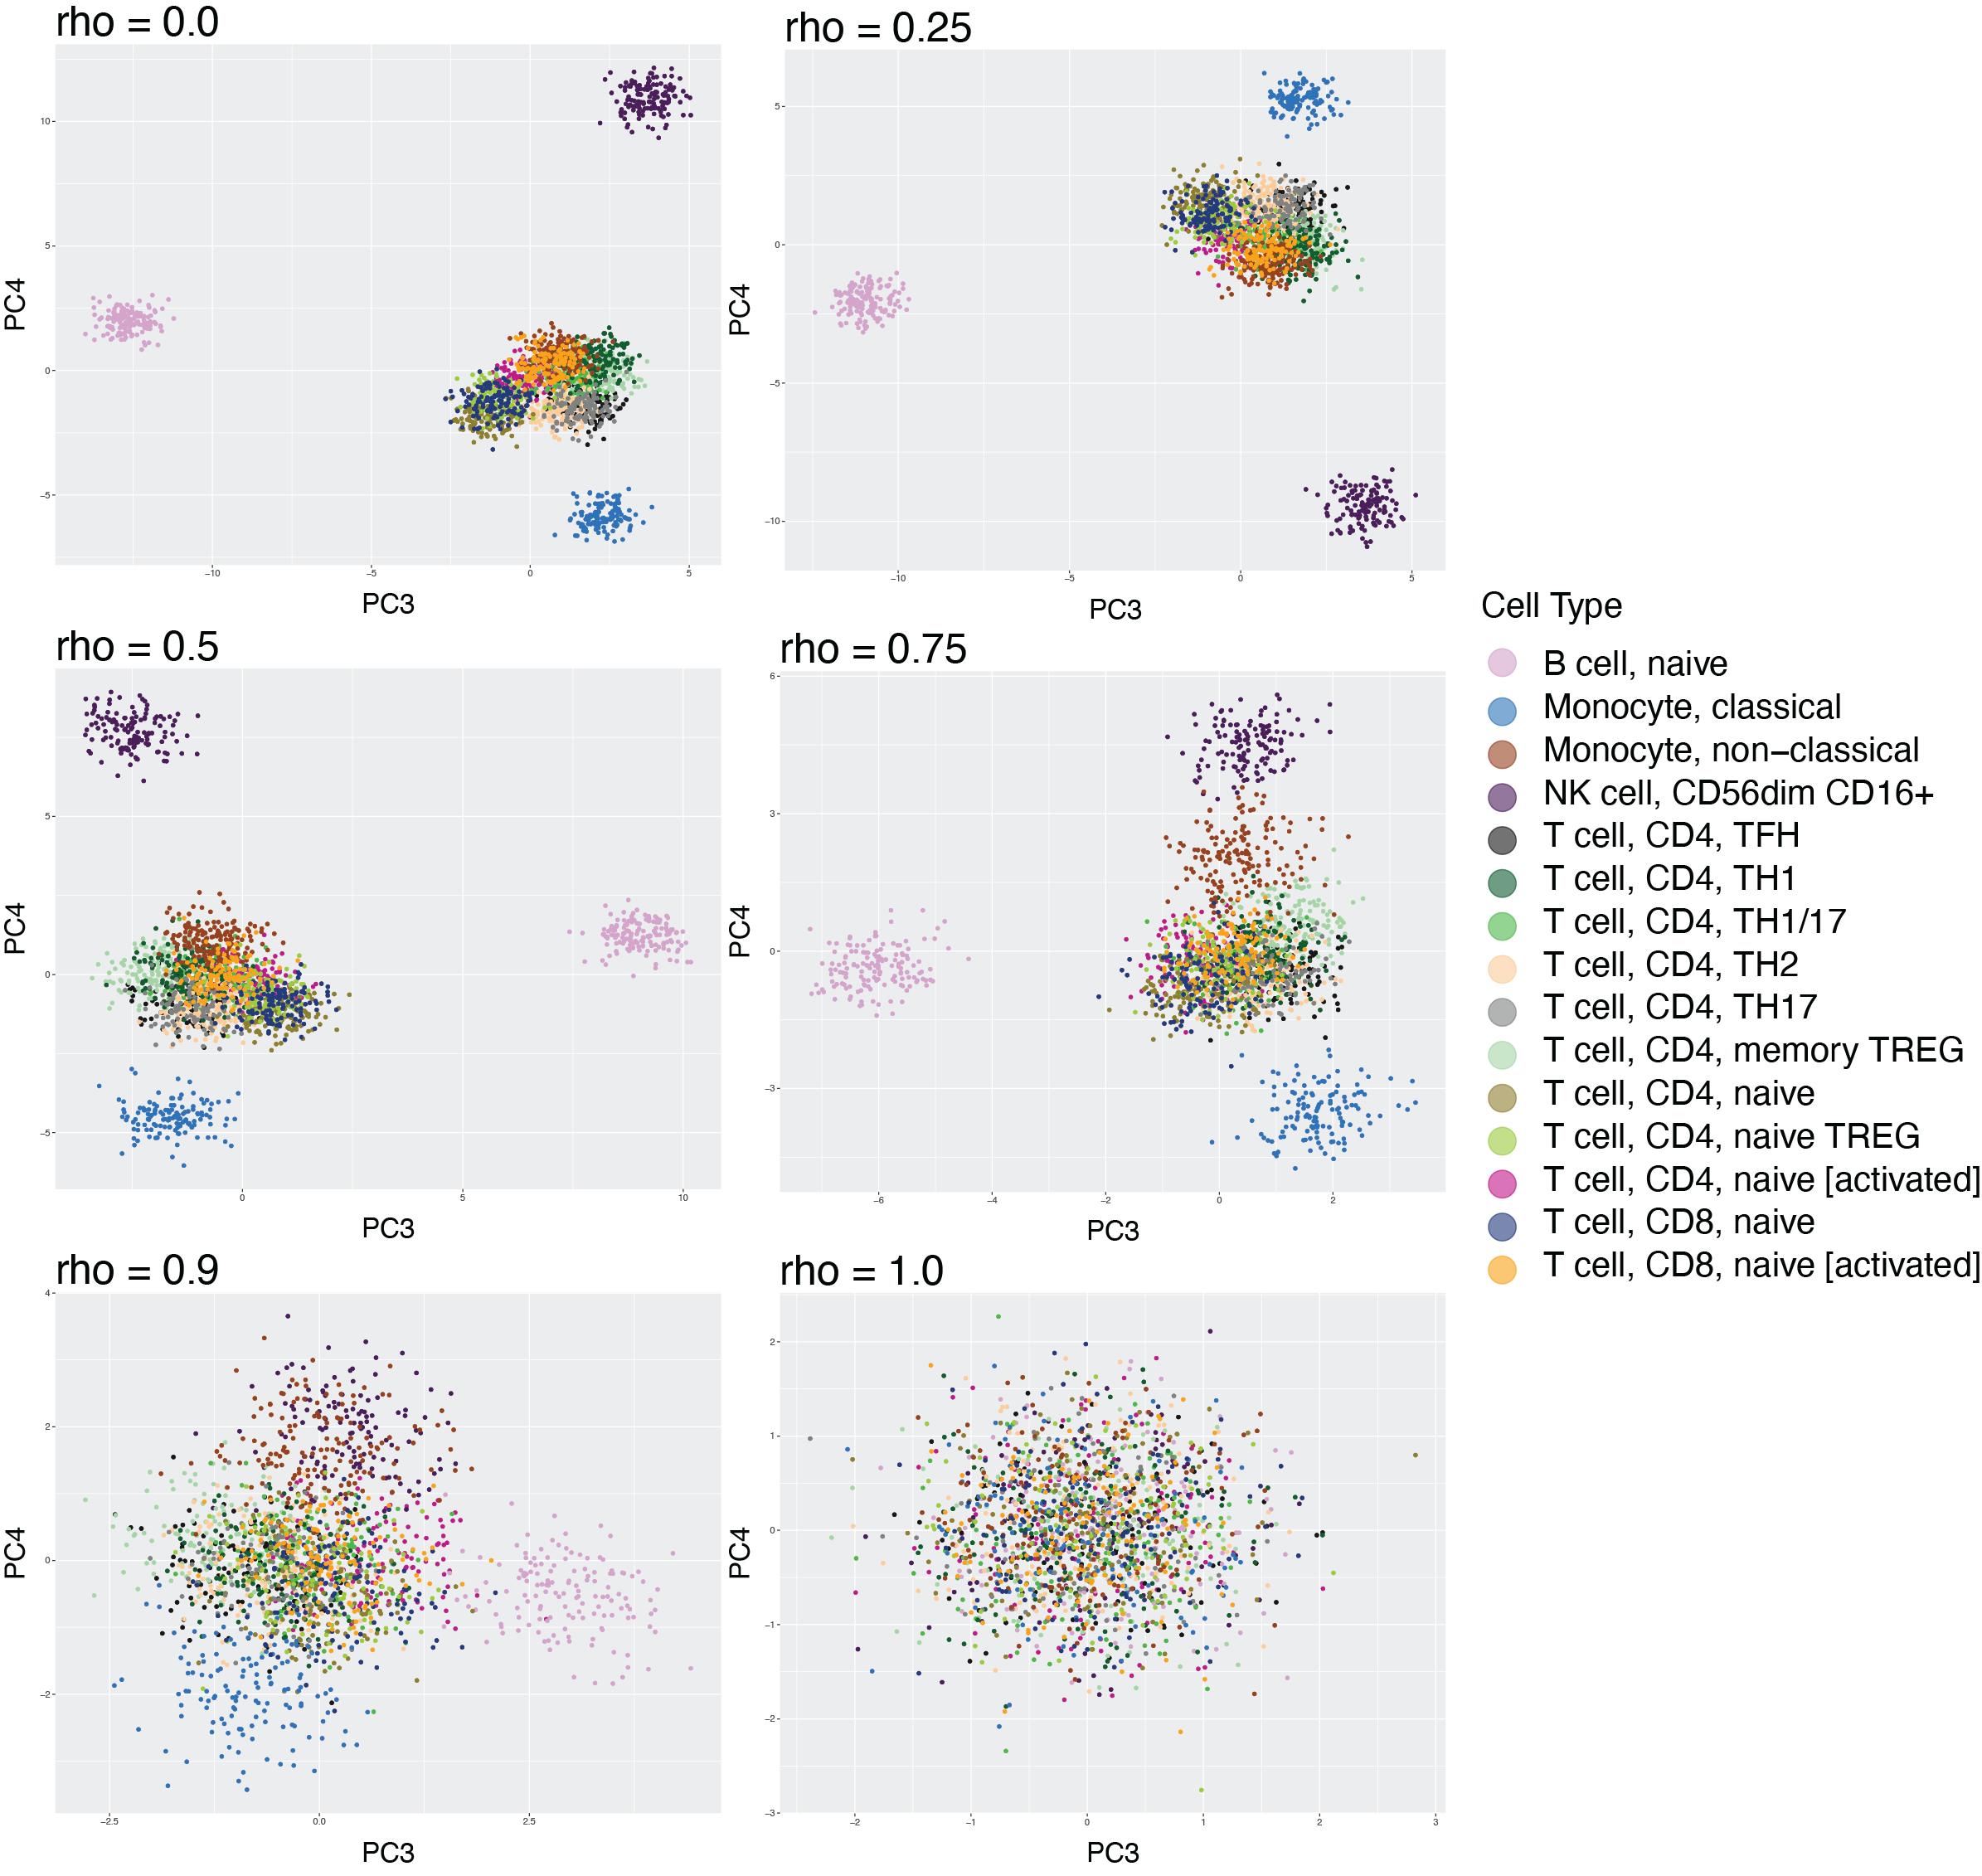
\includegraphics[width=\textwidth]{Figures/sim_data_PC34.png}
    \caption{\textbf{Simulated scRNA-seq datasets exhibit realistic distribution of expression patterns across various noise levels} Shown are the plots of third and fourth PCs for generated immune cell scRNA-seq datasets from the simulation scheme. Datasets generated using various noise proportions $\rho = \{0.0, 0.25, 0.5, 0.75, 0.9, 1.0\}$ are shown and coloured by cell type.}
    \label{fig:ct-pca-supp}
\end{figure}
\renewcommand{\arraystretch}{1}
\begin{table}[]
    \centering
    \begin{tabular}{|p{3cm}||p{4cm}|p{4cm}|}
    \hline
    Node & No. significantly upregulated genes & No. significantly downregulated genes\\
    \hline
    \multicolumn{3}{|c|}{Level 0}\\
    \hline
        \texttt{node\_0} & 0 & 157 \\
    \hline
    \multicolumn{3}{|c|}{Level 1}\\
    \hline
        \texttt{node\_1} & 525 & 242 \\        \texttt{node\_2} & 133 & 100 \\
    \hline
    \multicolumn{3}{|c|}{Level 2}\\
    \hline
        \texttt{node\_3} & 215 & 71 \\
        \texttt{node\_4} & 198 & 69 \\
        \texttt{node\_5} & 1705 & 289 \\
        \texttt{node\_6} & 485 & 123 \\
    \hline
    \multicolumn{3}{|c|}{Level 3}\\
    \hline
        \texttt{node\_7} & 1399 & 102 \\
        \texttt{node\_8} & 47 & 6 \\
        \texttt{node\_9} & 227 & 29 \\
        \texttt{node\_10} & 361 & 54 \\
        \texttt{node\_11} & 582 & 54 \\
        \texttt{node\_12} & 1451 & 160 \\
        \texttt{node\_13} & 677 & 74 \\
        \texttt{node\_14} & 280 & 63 \\
    \hline
    \multicolumn{3}{|c|}{Level 4}\\
    \hline
        \texttt{node\_15} & 830 & 16 \\
        \texttt{node\_16} & 823 & 56 \\
        \texttt{node\_17} & 41 & 3 \\
        \texttt{node\_18} & 49 & 2 \\
        \texttt{node\_19} & 1172 & 93 \\
        \texttt{node\_20} & 334 & 19 \\
        \texttt{node\_21} & 486 & 33 \\
        \texttt{node\_22} & 913 & 81 \\
        \texttt{node\_23} & 808 & 43 \\
        \texttt{node\_24} & 1185 & 100 \\
        \texttt{node\_25} & 764 & 59 \\
        \texttt{node\_26} & 1003 & 74 \\
        \texttt{node\_27} & 1096 & 102 \\
        \texttt{node\_28} & 894 & 44 \\
        \texttt{node\_29} & 286 & 7 \\
        \texttt{node\_30} & 638 & 87 \\
    \hline
    \end{tabular}
    \caption{\textbf{Table outlining the number of significant genes for each latent node} Upregulated genes are identified as genes with an embedding value of $\hat{\beta} > 0$ to a significance level of $\alpha = 0.05$. Inversely, downregulated genes are those with an embedding values of $\hat{\beta} < 0$. }
    \label{tab:sig_genes}
\end{table}

\begin{table}[]
    \centering
    \begin{tabular}{|p{3cm}||p{4cm}|p{4cm}|}
    \hline
    Node & No. unique significantly upregulated genes & No. unique significantly downregulated genes\\
    \hline
    \multicolumn{3}{|c|}{Level 0}\\
    \hline
        \texttt{node\_0} & 0 & 157 \\
    \hline
    \multicolumn{3}{|c|}{Level 1}\\
    \hline
        \texttt{node\_1} & 525 & 154 \\        \texttt{node\_2} & 133 & 40 \\
    \hline
    \multicolumn{3}{|c|}{Level 2}\\
    \hline
        \texttt{node\_3} & 188 & 19 \\
        \texttt{node\_4} & 183 & 19 \\
        \texttt{node\_5} & 1662 & 250 \\
        \texttt{node\_6} & 476 & 78 \\
    \hline
    \multicolumn{3}{|c|}{Level 3}\\
    \hline
        \texttt{node\_7} & 1394 & 88 \\
        \texttt{node\_8} & 38 & 1 \\
        \texttt{node\_9} & 213 & 14 \\
        \texttt{node\_10} & 344 & 17 \\
        \texttt{node\_11} & 292 & 31 \\
        \texttt{node\_12} & 995 & 41 \\
        \texttt{node\_13} & 622 & 26 \\
        \texttt{node\_14} & 249 & 26 \\
    \hline
    \multicolumn{3}{|c|}{Level 4}\\
    \hline
        \texttt{node\_15} & 429 & 12 \\
        \texttt{node\_16} & 620 & 8 \\
        \texttt{node\_17} & 37 & 1 \\
        \texttt{node\_18} & 45 & 1 \\
        \texttt{node\_19} & 1098 & 69 \\
        \texttt{node\_20} & 244 & 12 \\
        \texttt{node\_21} & 400 & 19 \\
        \texttt{node\_22} & 870 & 49 \\
        \texttt{node\_23} & 639 & 34 \\
        \texttt{node\_24} & 1022 & 61 \\
        \texttt{node\_25} & 214 & 22 \\
        \texttt{node\_26} & 445 & 24 \\
        \texttt{node\_27} & 959 & 49 \\
        \texttt{node\_28} & 687 & 30 \\
        \texttt{node\_29} & 229 & 5 \\
        \texttt{node\_30} & 608 & 44 \\
    \hline
    \end{tabular}
    \caption{\textbf{Table outlining the number of unique significant genes for each latent node} Upregulated genes are identified as genes with an embedding value of $\hat{\beta} > 0$ to a significance level of $\alpha = 0.05$. Inversely, downregulated genes are those with an embedding values of $\hat{\beta} < 0$. Genes are considered unique to a node if it does not also appear as a significant gene in its parent and sibling node.}
    \label{tab:unique_sig_genes}
\end{table}

\begin{figure}
    \centering
    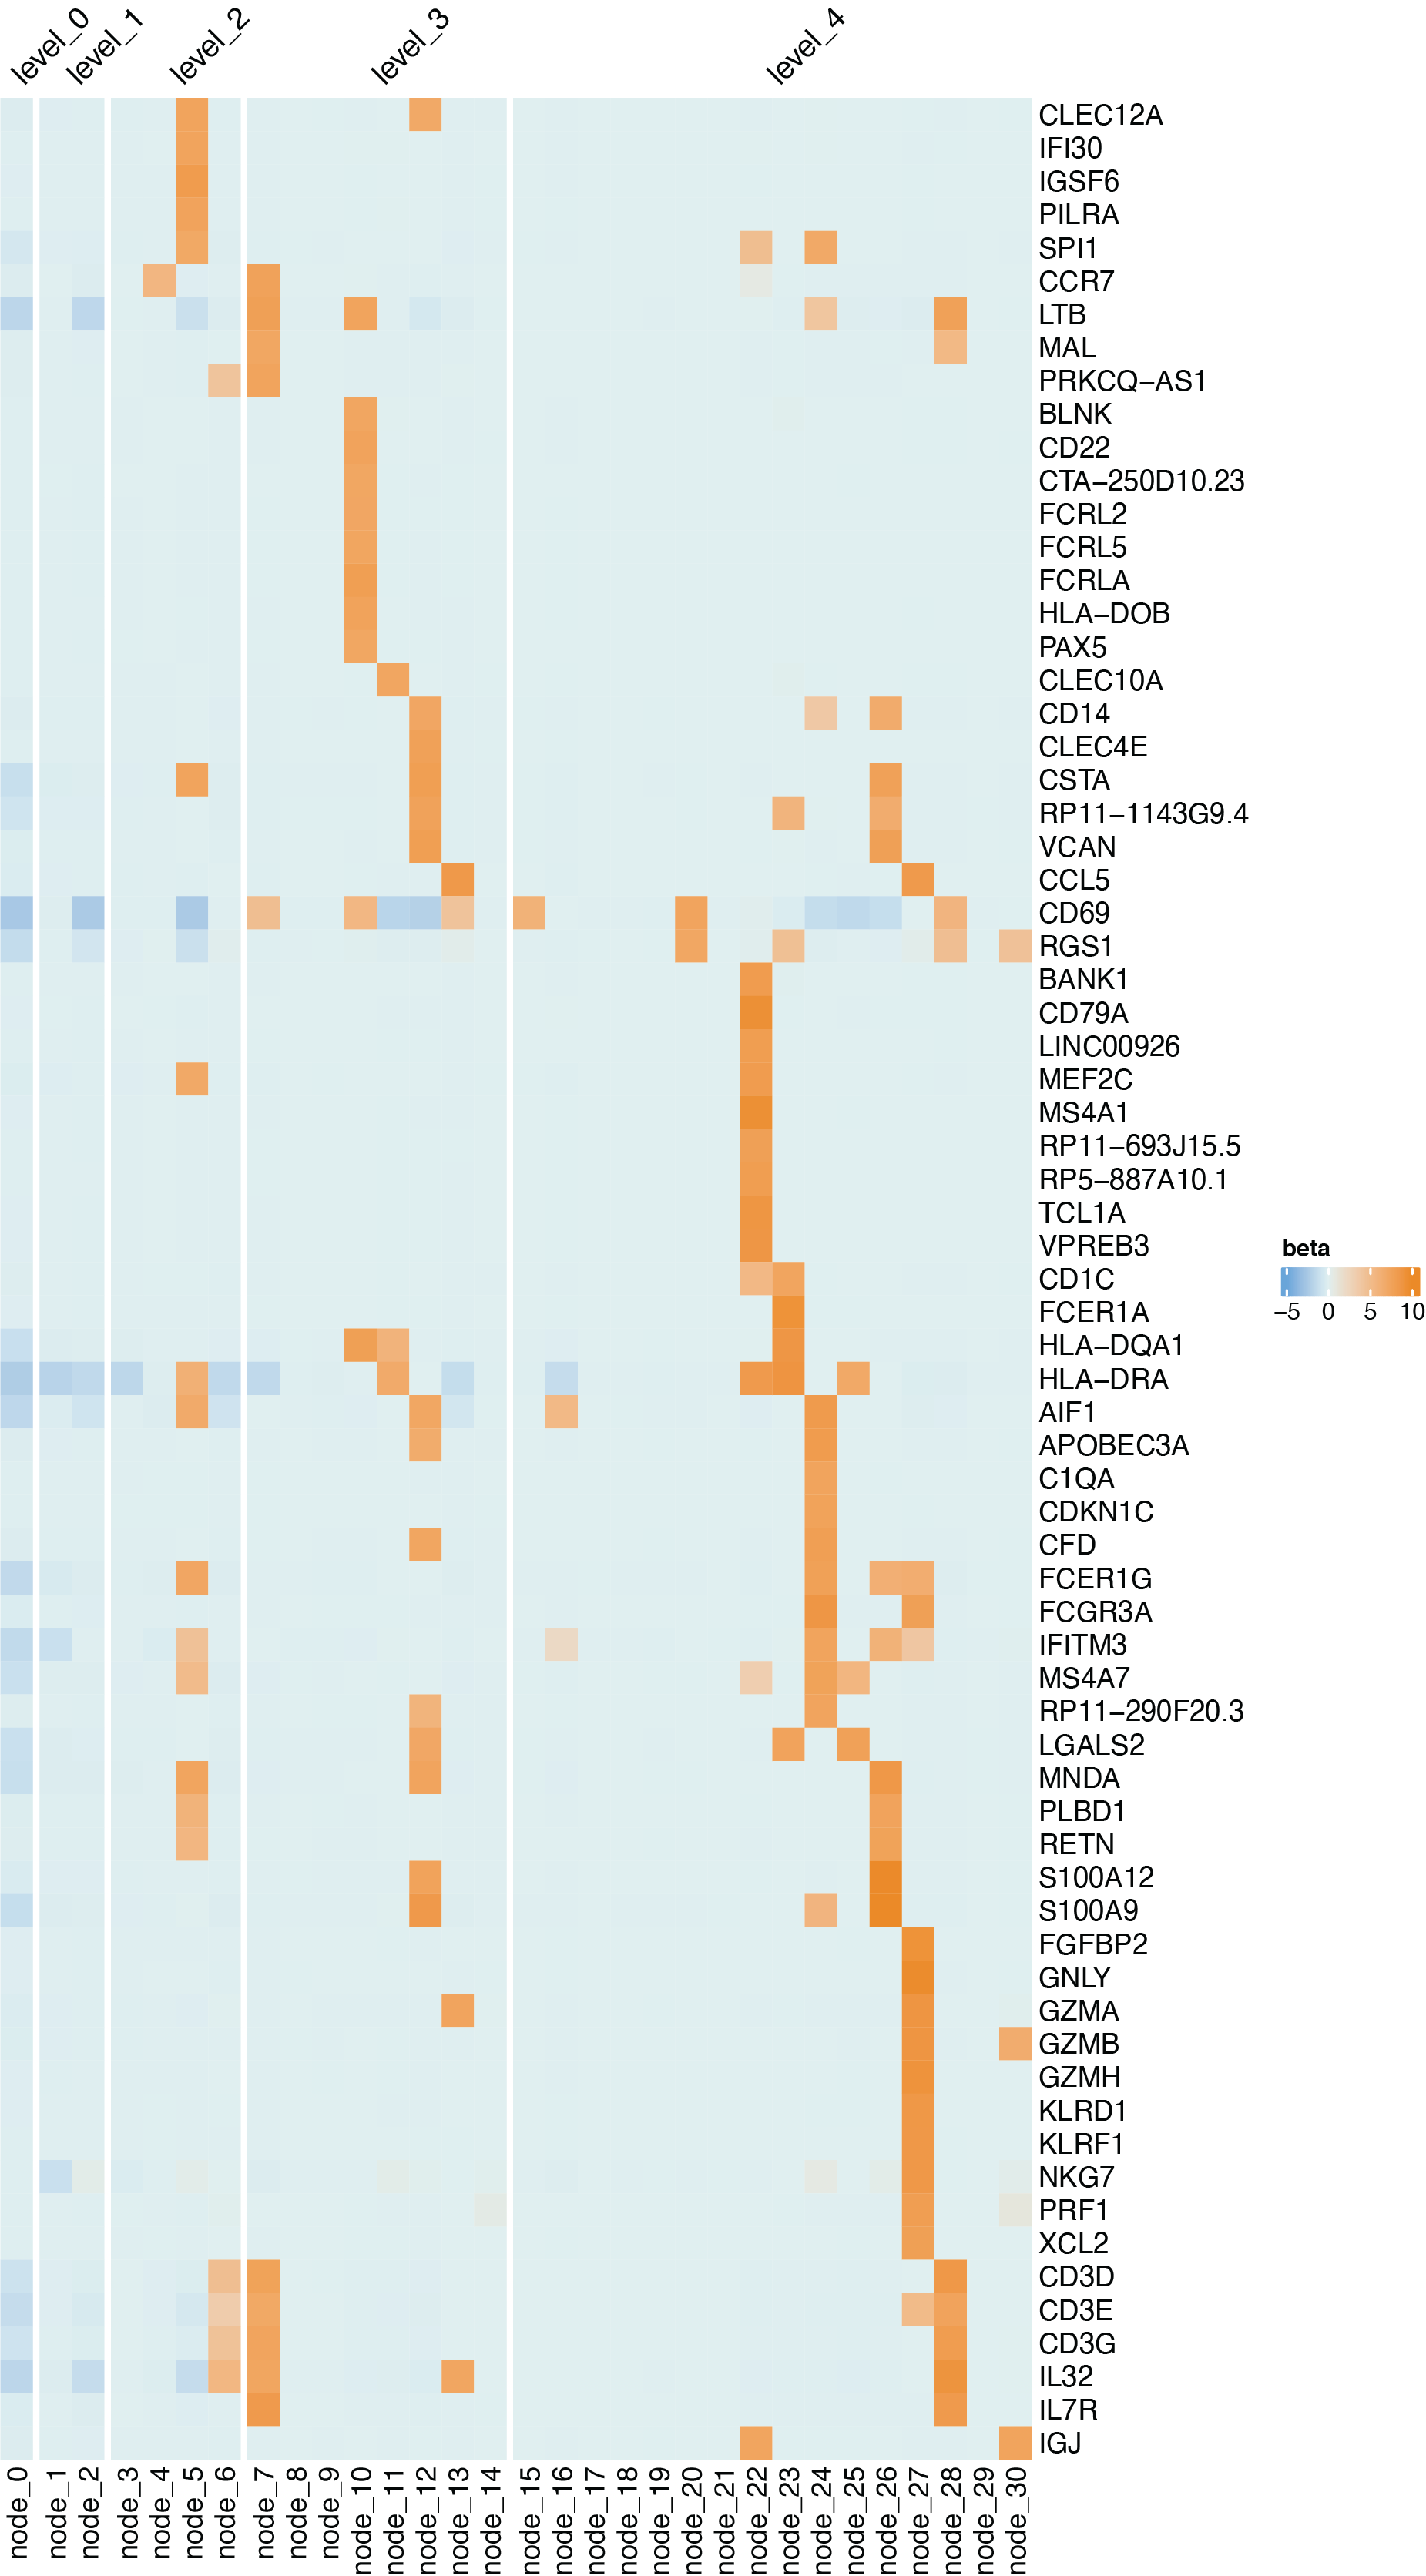
\includegraphics[scale=0.6]{Figures/top_beta_hm.png}
    \caption{\textbf{Heatmap of top genes shows candidates for further analysis} Heatmap shows estimated gene embedding values $\hat{\beta}$ of top genes across all latent tree nodes. Genes are selected as the 80 gene with the greatest absolute $\hat{\beta}$ values amongst the aggregated pool of the top ten genes per latent tree node.}
    \label{fig:top_beta_hm}
\end{figure}

\begin{figure}
    \centering
    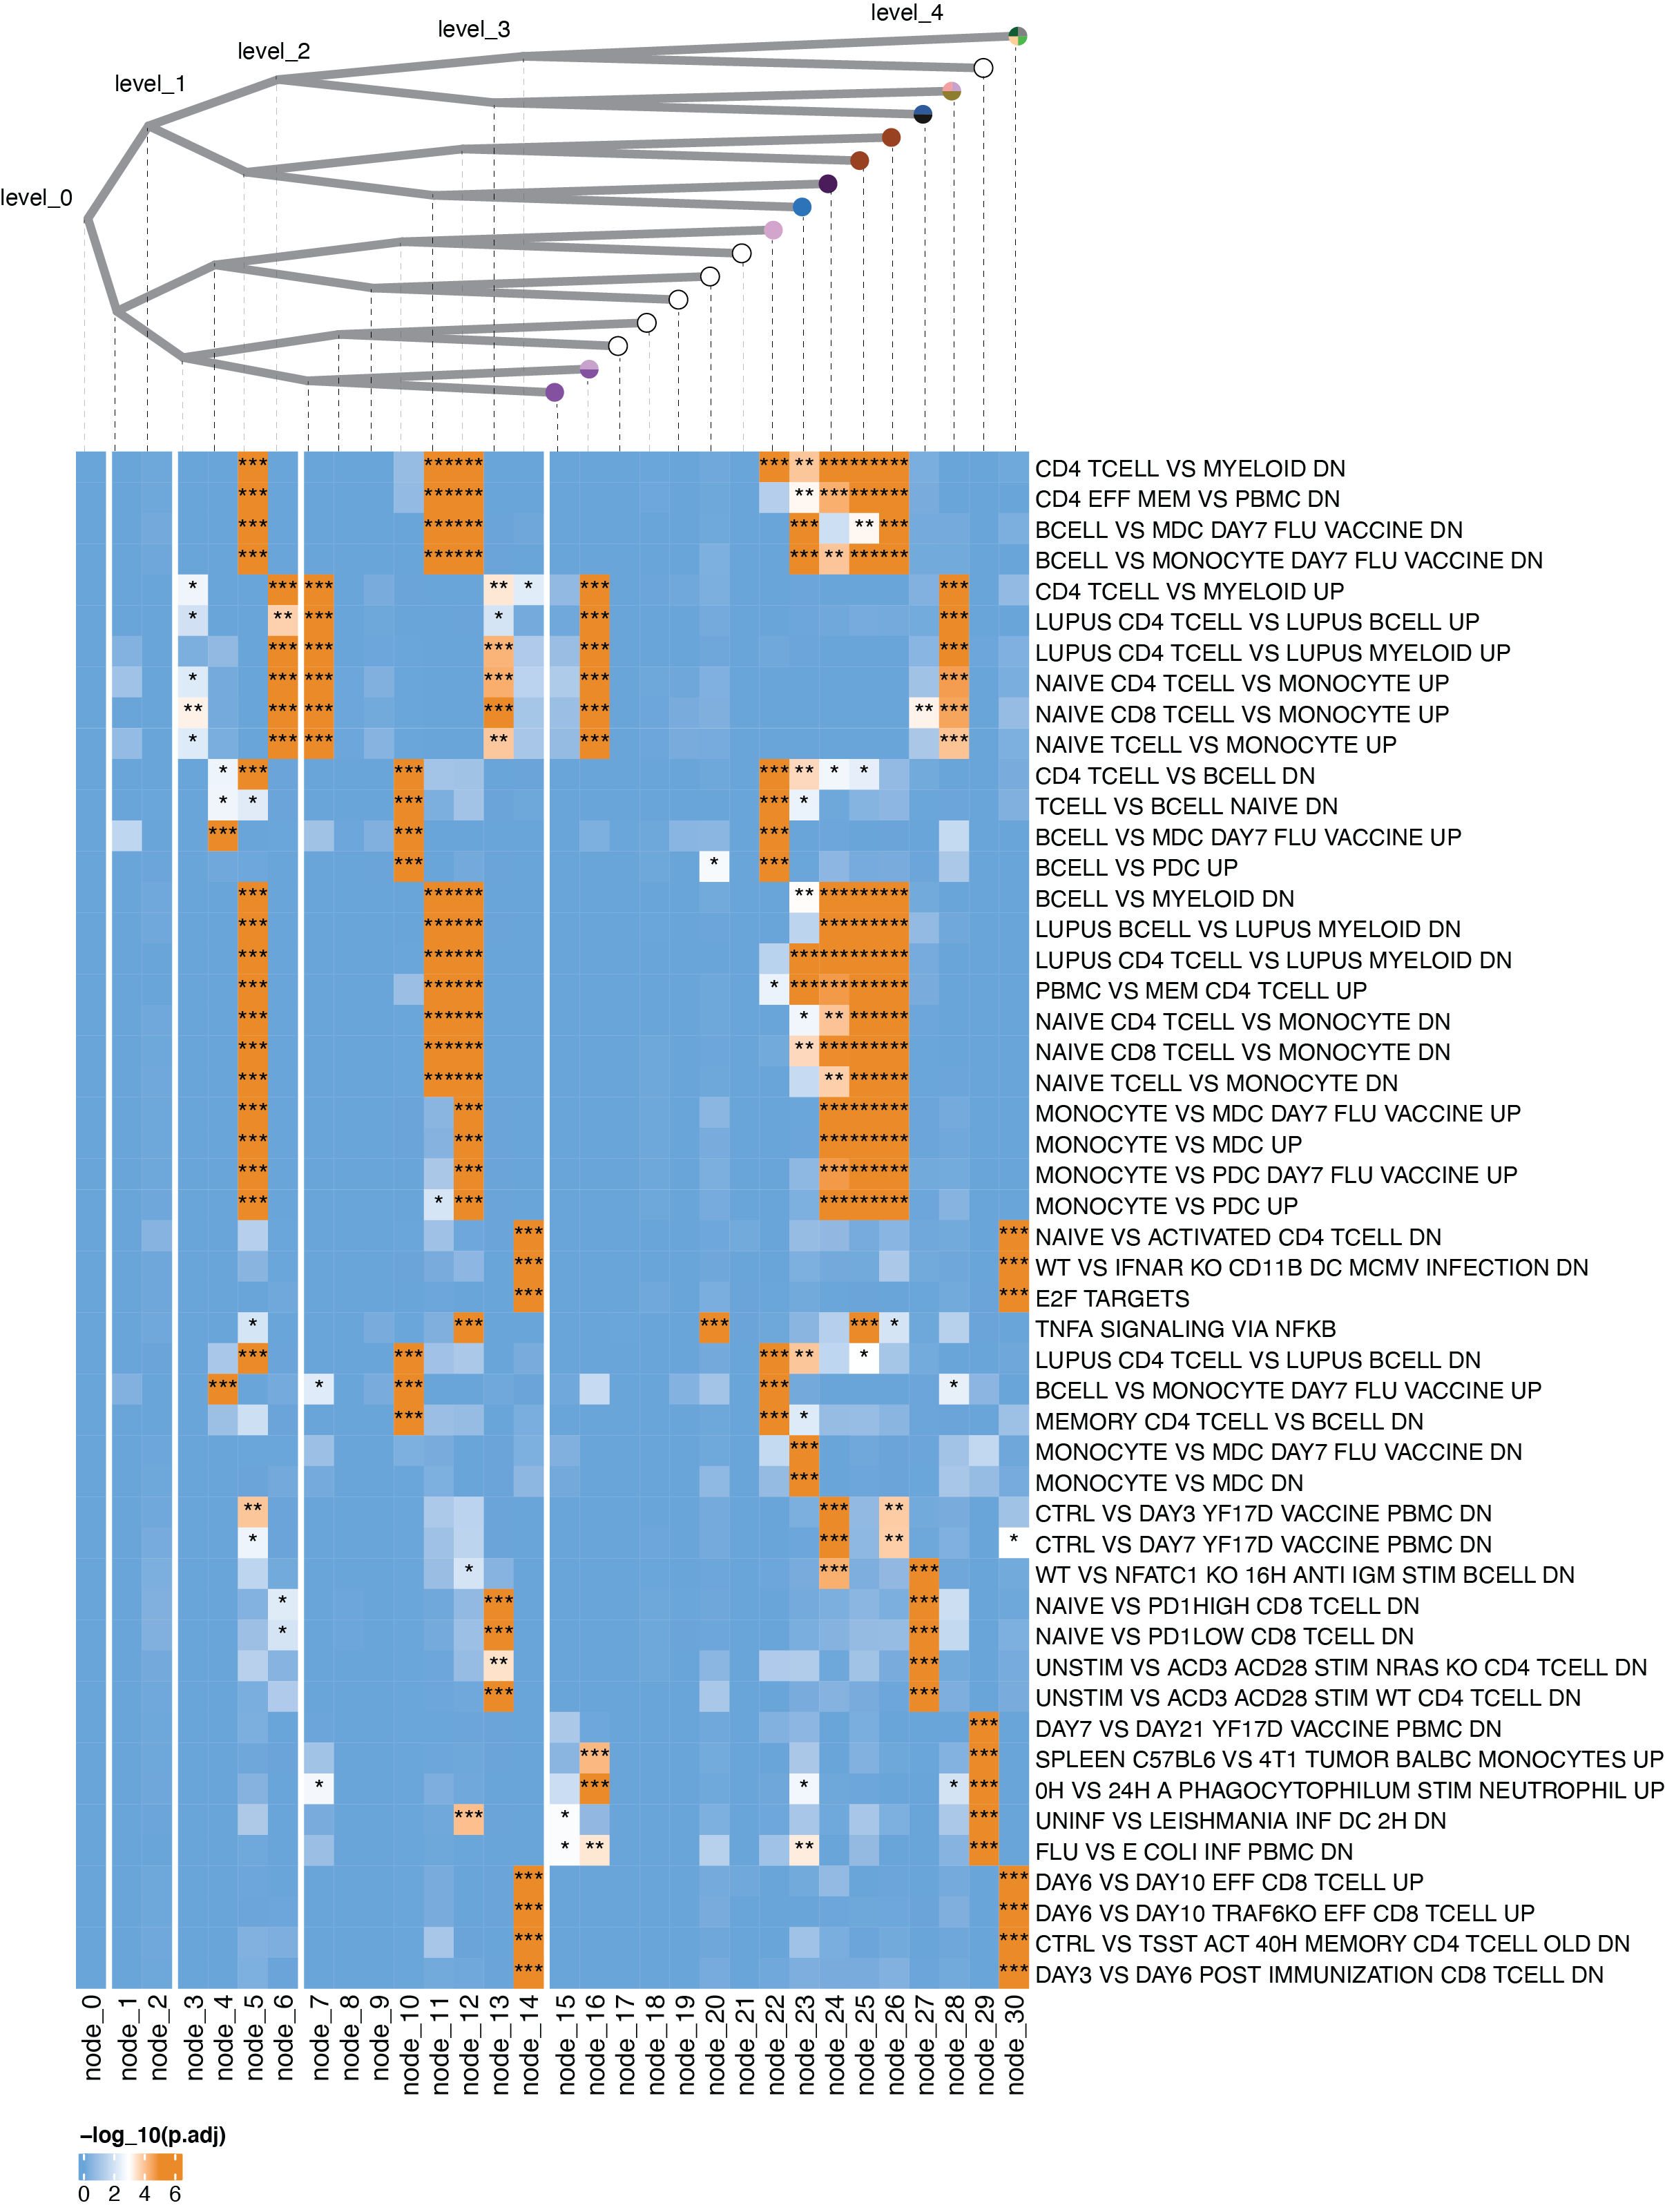
\includegraphics[scale=0.65]{Figures/immune_gsea.png}
    \caption{\textbf{Enrichment analysis of gene sets related to immune function show cell function described by latent node embeddings} Heatmap shows the $-\log(p)$ enrichment significance of each gene set per node. Significance annotations are as follows: $*** - p < 0.0001, ** - p < 0.001, * - p < 0.01$}
    \label{fig:immune_gsea}
\end{figure}

